% Art der Arbeit: Bachelorarbeit
% Titel: "BLAST Avionics Thermal Management"
% Autor: Viktor Hoffmann
%-----------------------------------------------------------------------------------
% verwendete Packages
\documentclass{ITLR}
% Use ITLR.cls for first style-definition. 
% IMPORTANT: change in ITLR.cls colors in hyperref-package ONLY for printing; NOT for PDF submittance


% ----------- Zusätzliche Usepackages ----------------------------------------------
% Hier stehen weitere Usepackages ...
\usepackage{siunitx}
\usepackage{tikz}
\usepackage{subcaption}
\usetikzlibrary{arrows.meta}
\usepackage{acronym}
\usepackage{pdfpages}
\usepackage{booktabs}

% ----------- Graphics Paths -------------------------------------------------------
\graphicspath{{Bilder/}}

%###################################################################################
% ----------- Dokumentanfang -------------------------------------------------------
\begin{document}
\setstretch{1.1667} 		% Zeilenabstand (Verhältnis, hier z.B. 14pt/12pt)
\pagestyle{Abstract}		% oben definiert

% ----------- Title & Preface  -----------------------------------------------------
\pagenumbering{Alph}
%\begin{titlepage}
%---- ITLR-Logo ----
\begin{figure}[ht]
     \centering
      \includegraphics[width=65mm]{./Logos/ITLR_Logo.eps}
\end{figure}

\hspace{200mm}

%---- Title of the study thesis ----
\begin{center}
    \begin{Large}
        Bachelorarbeit
    \end{Large}

    \vspace{2.5mm}

    \BRule
    \vspace{2.5mm}
    \begin{LARGE}
    \\
        Entwicklung des Avionik-Thermal-Managements einer Experimentalrakete
        \\
    \vspace{1mm}
    \end{LARGE}
    \vspace{2.5mm}
    \BRule
    \vspace{15mm}

    \begin{Large}

    Viktor Hoffmann \\
    
\end{Large}

\end{center}

\vfill

%---- Uni-Logo ----
\begin{wrapfigure}[4]{l}{17mm}
    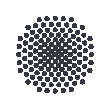
\includegraphics[width=17mm]{./Logos/unilogo_neu}
\end{wrapfigure}

\parbox[t]{120mm}
{
    \sffamily
      \vspace{3mm}
        Universität~Stuttgart\\
        \textbf{Institut~für~Thermodynamik~der~Luft-~und~Raumfahrt~(ITLR)}\\[2mm]
        Direktor: Prof.~Dr.-Ing.~habil.~Bernhard~Weigand
}




\end{titlepage}

\includepdf{Text/Hoffmann_BA_Deckblatt2.pdf}
\newpage\null\thispagestyle{empty}\newpage
\includepdf{Text/Aufgabenstellung_BA_Hoffmann.pdf}
\includepdf{Text/Hoffmann_Bachelor_Eidesstatt.pdf}
\includepdf{Text/Hoffmann_BA_Erklärung_Archivierung.pdf}

% erste Seite: Titelblatt (wird von ITLR erstellt)
% zweite Seite: leeres Blatt
% dritte Seite: Aufgabenstellung (wird von ITLR erstellt)
% vierte Seite: Erklärung (wird von ITLR erstellt, muss aber noch unterschrieben werden)

\pagenumbering{Roman}		% Am Anfang römische Seitenzahlen
% ----------- Abstract -------------------------------------------------------------
\newpage
\phantomsection		% Korrigiert die Hyperref-Verlinkungen
\addcontentsline{toc}{chapter}{Kurzzusammenfassung} %\addcontentsline
\chapter*{Kurzzusammenfassung} % * means not in table of content
\label{chap:Kurzzusammenfassung}

% ca. 150 Worte / Aufgabenstellung, Zielsetzung, verwendete Methoden, Ergebnisse kurz vorstellen, aber nicht diskutieren / Leser entscheidet hier, ob er die Arbeit für lesenswert hält

% deutsch
Für das Projekt \ac{blast} der Hochschulgruppe \ac{hyend} wird eine neue, kompakte und hochleistungsfähige Avionik entwickelt,
die unter extremen Flugbedingungen arbeitet. Die in dieser Arbeit entwickelte Kühlung muss leicht, ausfallsicher und für eine
maximale Sperrschichttemperatur von $T_\mathrm{J} \approx T_\mathrm{C} \leq \SI{85}{\celsius}$ für die gesamte Missionsdauer ausgelegt sein.
Basierend auf den Anforderungen und einer Trajektoriensimulation
wurden drei Konzepte untersucht: reiner Radiator, reines \ac{pcm} und eine hybride Radiator-\ac{pcm}-Lösung. Die Vorauslegung
ergab, dass ein Radiator wegen aerothermaler Aufheizung ungeeignet ist. Die hybride Lösung ist möglich, jedoch durch geometrische
Verluste und hohe Luftwärmeströme der Vorauslegung nach mit \SI{3.835}{\kilogram} schwerer als ein einfaches \ac{pcm}
mit \SI{0.316}{\kilogram}. \ac{cht}-Simulationen der Außenströmung und des \ac{pcm}
bestätigten trotz angenommener Vereinfachungen die Vorauslegungsergebnisse mit einer Masse des hybriden Radiator-\ac{pcm} von \SI{1.522}{\kilogram}.

\chapter*{Abstract} % * means not in table of content
\label{chap:Abstract}
Advanced avionics systems are essential to the success of any experimental rocket.
Ranging from flight computers, telecommunications, and data acquisition to the control
of onboard instrumentation and the rocket itself, high-power microelectronics play a critical role and are often implemented with redundancy.
These systems must be highly compact and capable of withstanding demanding flight conditions, which lead to elevated
power densities that, if not properly managed, can significantly reduce operational lifetime or even cause premature mission failure.
Such is the case in the project \ac{blast} where a novel avionics system is being developed by \ac{hyend} and in need of a thermal management solution.\\

In a first step the demands on the thermal management were set to a maximum junction temperature

% ----------- Verzeichnisse --------------------------------------------------------
% Inhaltsverzeichnis, Abbildungsverzeichnis, Tabellenverzeichnis, Nomenklatur 
\newpage
\tableofcontents	% Erstellt automatisch die Überschrift "Inhaltsverzeichnis" mit

% Tabellenverzeichnis
\newpage
\phantomsection		% Korrigiert die Hyperref-Verlinkungen
\pagestyle{VerzeichnisseNomenklatur}		% wie oben definiert
\addcontentsline{toc}{chapter}{Tabellenverzeichnis} 	% Eintrag ins InhaltsVZ
\listoftables

% Abbildungsverzeichnis
\newpage
\phantomsection		% Korrigiert die Hyperref-Verlinkungen
\addcontentsline{toc}{chapter}{Abbildungsverzeichnis}
\listoffigures				

% Symbolverzeichnis
\newpage
\phantomsection		% Korrigiert die Hyperref-Verlinkungen
\addcontentsline{toc}{chapter}{Symbolverzeichnis}
\chapter*{Symbolverzeichnis}
	
\subsection*{Lateinische Symbole}

\begin{supertabular}{p{10mm}p{3mm}p{20mm}p{3mm}l}
$T$ && \SI{}{\kelvin} && Temperatur\\
$c$ && \SI{}{\joule\per\kilogram\per\kelvin} && Spezifische Wärmekapazität\\
$h$ && \SI{}{\joule\per\kilogram} && Spezifische Schmelzenthalpie\\
\end{supertabular}


\subsection*{Griechische Symbole}

\begin{supertabular}{p{10mm}p{3mm}p{20mm}p{3mm}l}
$\rho$ && \SI{}{\kilogram\per\cubic\meter} && Dichte\\
$\lambda$ && \SI{}{\watt\per\meter\per\kelvin} && Wärmeleitfähigkeit\\
$\gamma$ && \SI{}{\per\kelvin} && Wärmeausdehnungskoeffizient\\
$\epsilon$ && && Emissionsgrad\\
$\alpha$ && && Absorptionsgrad\\
\end{supertabular} 

\subsection*{Indizes}

\begin{supertabular}{p{10mm}p{3mm}p{20mm}p{3mm}l}
solidus && && Solidus Temperatur des Phasenwechsels\\
liquidus && && Liquidus Temperatur des Phasenwechsels\\
solid && && Feststoff Eigenschaften\\
liquid && && Flüssigstoff Eigenschaften\\
fus && && Schmelz Phasenwechsel\\
p && && Konstanter Druck\\
J && && Sperrschicht\\
C && && Gehäuse\\
safety && && Mit Sicherheitsfaktor 1.5\\
t && && spektral integriert\\
s && && solar\\
\end{supertabular} 

\subsection*{Konstanten}

\begin{supertabular}{p{10mm}p{3mm}p{50mm}p{3mm}l}
$\pi$ && $\approx \SI{3.142}{\kelvin}$ && Kreiszahl\\
$\sigma$ && $\approx \SI{3.67e-8}{\watt\per\meter\squared\per\kelvin\tothe{4}}$ && Stefan-Boltzmann-Konstante\\
\end{supertabular}

\newpage

%---Akronyme
\subsection*{Abkürzungen}
\begin{acronym}[BLAST]
\acro{pcm}[PCM]{Phase Change Material}
\acro{pcb}[PCB]{Printed Circuit Board}
\acro{blast}[BLAST]{Biliquid launch and Space Technology}
\acro{fcc}[FCC]{Flight Control Computer}
\acro{hyend}[HyEnD]{Hybrid Engine Development}
\acro{cfd}[CFD]{Computational Fluid Dynamics}
\acro{cht}[CHT]{Conjugate Heat Transfer}
\acro{pgs}[PGS]{Pyrolithic Graphite Sheet}
\acro{maxq}[max~Q]{Maximaler dynamischer Druck}
\acro{gse}[GSE]{Ground Support Equipment}
\acro{pcdu}[PCDU]{Power Control and Delivery Unit}
\acro{atm}[ATM]{Avionik-Thermal-Management}
\acro{rom}[ROM]{Reduced Order Model}
\acro{udf}[UDF]{User Defined Function}
\end{acronym}

% ----------- Verzeichnisse Ende-----------------------------------------------------
\newpage
\pagestyle{main}			% ab hier: normale Kopf- und Fußnoten
% ----------- Einleitung ------------------------------------------------------------
\chapter{Einführung}			
\label{sec:Introduction}
\pagenumbering{arabic}		%ab hier: arabische Seitenzahlen (Hauptteil)

% Problemstellung und Lösungsansätze, 2-3 Seiten / keine Ergebnisse & Folgerungen /

Die Avionik ist ein Grundstein jeder erfolgreichen Experimentalrakete. Ob es hierbei um Telekommunikation,
Datenerfassung oder auch aktive Steuerung und Regelung von
Instrumenten und dem Fahrzeug während des Flugs geht, kompakte Hochleistungsmikroelektronik ist immer gefragt und muss oft redundant ausgeführt sein.
Diese Elektronik, die zudem noch extremen Bedingungen ausgesetzt wird, kommt jedoch mit einer
substanziellen Wärmeleistung und Wärmestromdichte die, bei mangelhafter Rücksicht zu reduzierter Lebensdauer der Avionik führt,
oder sogar die Mission frühzeitig scheitern lässt.\\

Diese Arbeit befasst sich mit der lösung des dargestellten problems für das Projekt \ac{blast} der studentischen Hochschulgruppe \ac{hyend}
wo eine neue Avionik entwickelt wird und ein \ac{atm} benötigt wird.

\section{Darstellung des Problems}

Das Thermal-Problem einer Experimentalrakete beginnt bereits lange vor dem eigentlichen Start. Oft muss nach integration und
Befestigung der Rakete auf der Rail und Verbindung mit dem \ac{gse} noch einige Stunden auf das Startfenster gewartet werden.
Während dieser Zeit steht die Rakete der Umwelt ausgesetzt oft in der Sonne und kann, je nach Struktur und Beschichtung der Sektion 
interne Temperaturen über den zulässigen \SI{89.15}{\degreeCelsius} erreichen. Da in dieser Phase eine Verbindung mit dem 
\ac{gse} besteht kann Masse durch externe Kühlung währenddessen eingespart werden, weshalb in dieser Arbeit nur für die darauf folgende 
Flugphase das \ac{atm} entwickelt werden soll.
Da \ac{blast} für ein Apogäum über der Kármán-Linie (\SI{100}{\kilo\meter}) entwickelt wird, sind während dem Flug extreme Umweltbedingungen
durch aerothermale Aufheizung, microgravitation und annäherndes Vakuum zu erwarten, die ein komplexes \ac{atm} fordern.\\

In der Vergangenheit wurde bei \ac{hyend} oft die Avionik ohne Redundanz oder zusammen mit fertig gekaufter Avionik, für 
Missionskritische Aufgaben wie den Fallschirm-Auswurf, ausgeführt. Beim Projekt \ac{blast} soll das vermieden werden, 
indem der selbst entwickelte \ac{fcc} in Dual Duplex Redundanz ausgelegt wird. Demensprechend gibt es vier Computer die
die selben Programme ausführen und den vierfachen Stromverbrauch gegenüber einfach ausgeführter Avionik haben. Hinzu kommen
weitere Kameras, Funkplatinen, Verstärker, Sensor-Schnittstellen etc. die jedoch keine redundante Ausführung haben.\\

Dem Energieerhaltungssatz nach haben der \ac{fcc}, die Kameras und weitere Elektronik die keine Leistung abgibt, gegenüber etwa
der \ac{pcdu} und Funkplatine welche Leistung in Form von Strom und elektromagnetischer Strahlung abgeben, einen Wirkungsgrad von
\SI{0}{\percent}, da Logikoperationen physikalisch gesehen keine Arbeit sind. Resultierend wird der komplette Stromverbrauch
in Wärme umgewandelt.

\section{Zielsetzung der Arbeit}

Da es sich beim \ac{atm} um ein peripheres System handelt, soll besonders hohe Zuverlässigkeit gewehrleistet werden, da trotz der
Redundanz des \ac{fcc} ein Ausfall der Kühlung zum Ausfall durch Überhitzung führen kann.\\
Desweiteren ist Wiederverwendbarkeit, die kosten minimiert, aber besonders komplexe Integrations- und Vorbereitungsvorgänge
vermeided eine Priorität.\\
Als letzte Anforderung, nach einer Auswahl basierend auf den ersten beiden, soll wegen des begrenzten Massenbudgets der Avionik
besonders auf Leichtbau geachtet werden und die Masse des \ac{atm} soweit wie möglich minimiert werden.\\

\section{Lösungsweg}

Um ein geeignetes \ac{atm} zu entwickeln wird zunächst eine Auswahl an etablierten Lösungen aus der Luft- und Raumfahrtindustrie
getroffen, die die gestellten Anforderungen erfüllen können.\\

Diese werden in der Vorauslegung mithilfe eines \ac{rom} in Python ausgewertet, um eine erste Abschätzung der Leistungsfähigkeit zu erhalten.\\
Anschließend wird die Vorauslegung, soweit mit vorhandenen Rechenressourcen möglich, durch \ac{cht}-Simulationen mit Domänenreduktion
verifiziert und vergleichbar gemacht.

%----------- Literaturrecherche -----------------------------------------------------
\newpage
 \chapter{Grundlagen}
\label{chap:Grundlagen}			% durch \label{} später auf Element verweisen

In diesem Kapitel werden die Thermodynamischen, Chemischen und Numerischen Grundlagen erläutert, die in dieser Arbeit angewandt wurden. 
% Bücher, aber auch Paper etc. 

\section{Sensible Wärme}\label{sec:sensiblewaerme}

Unter sensibler Wärme versteht man die Eigenschaft von Masse Energie zu absorbieren, oder abzugeben und dadurch die Temperatur zu ändern. Dieses
Phänomen kann durch die Änderung der kinetischen Energie von den molekularen Teilchen im System erklärt werden. Durch das einführen von Energie in
ein System steigt die kinetische Energie der Teilchen, welche diese Energie über molekurare Interaktionen verteilen:

\begin{equation}
    c = \frac{\Delta Q}{m \cdot \Delta T}
\end{equation}

Da Elektrionik eine gewisse Eigenmasse hat und meist Teil einer größeren Baugruppe ist, gibt es durch die Sensible Wärme eine Dämpfung
zu Temperaturänderungen, welche jedoch zeitlich von der Wärmeleitfähigkeit der Materialien abhängt.

\section{Latente Wärme}\label{sec:latentewaerme}

Im kontrast zur sensiblen Wärme ist latente Wärme, auch Umwandlungsenthalpie genannt, die Eigenschaft von Masse bei einem Phasenwechsel Energie
zu absorbieren oder abzugeben, ohne dass dabei die Temperatur sich ändert. Das ist durch die erhöhung der potentiellen Energie der Teilchen,
statt der kinetischen wie bei der sensiblen Wärme, zu verstehen. Effektiv erhöht sich also nicht die Geschwindigkeit der Teilchen sondern die
Anzahl an Stellen an die die Teilchen sich bewegen können.

\begin{equation}
    h = \frac{\Delta Q}{m}
\end{equation}

Da die latente Wärme für die meisten Materialien im Fest-Flüssig Übergang um mindestens den Faktor 10 größer ist als die sensible Wärme bei
einem Grad Temperaturerhöhung, kann diese sehr gut zur Absorption von überschüssiger Wärme über längere, aber finite, Zeiträume verwender werden,
wobei auch hier die Wärmeleitfähigkeit eine entscheidende Rolle bei der Umsetzung spielt.

\section{Wärmestrahlung}\label{sec:radiator}
Die Wärmestrahlung ist einer von drei Wegen, wie sich Wärme in einem System verteilt.

\begin{equation}
    Q=\sigma\epsilon A T^{4}
\end{equation}

\section{Hybrid Lösung}
\label{sec:hybridloesung}

\newpage


% ----------- Methodik --------------------------------------------------------------
\chapter{Vorauslegung}
\label{chap:Vorauslegung}
% Ziel hier: den Leser in die Lage versetzen, die wesentliche Struktur der Arbeit nachvollziehen zu können (Vorgehen / Geräte / Materialien / Verfahren [also auch Software]  / getroffene Annahmen ... sollten hier erklärt werden)
Die Vorauslegung basiert auf einer Trajektoriensimulation aus OpenRocket, welche vom Triebwerks-Subsystem durchgeführt wurde.
Diese Flugdaten~(\ref{fig:flugdaten_trajektoriensimulation}) sind eine Maximalabschätzung der Schubkraft und dauer, welche in maximaler Flugdauer und Aerodynamischen Aufheizung
resultiert.

\section{Anforderungen}

Da die Kühlung zeitgleich zu der Avionik entwickelt wurde, musste auf eine genaue Analyse aller Komponenten der Avionik verzichtet werden.
Stattdessen wurde anhand des bereits festgelegten Microcontrollers STM32H743ZGT6, der auf den redundanten Flugcomputern verwendet wird,
die Auslegung durchgeführt.\\
Aus dem Datenblatt des Microcontrollers folg eine maximale Sperrschichttemperatur von $T_\text{J} = \SI{125}{\degreeCelsius}$ und $T_\text{A} = \SI{85}{\degreeCelsius}$~\cite{STM32}
und ein Sperrschicht-Gehäuse Wärmeleitwiederstand von $\Theta_\text{JC} = \SI{23.9}{\degreeCelsius\per\watt}$. Mit einem konservativen
Sicherheitsfaktor von 1.5, um bisher unbekannte Bauteile zu berücksichtigen, folgt daraus $\Theta_\text{JC,safety} = \SI{35.85}{\degreeCelsius\per\watt}$
und eine maximale Gehäusetemperatur von $T_\text{C} = \SI{89.15}{\degreeCelsius}$.\\

Die Kühlung soll außerdem eine hohe Zuverlässigkeit haben, welche durch Verwendung von ausschließlich passiven Bauteilen gewehrleistet wird.
Dadurch kann aufwendiges und teures testen und verifizieren von aktiven Bauteilen mit mechanischer oder elektrischer Funktion vermieden werden und es besteht bei
nicht nominalen Flügen eine geringere Ausfallwahrscheinlichkeit durch die inherent größeren Toleranzen passiver Bauteile.

\begin{figure}[H]
    \centering

    % Column 1, Row 1
    \begin{subfigure}{0.48\textwidth}
        \centering
        \includegraphics[width=\linewidth]{../../Code/acceleration_over_time.pdf}
        \caption{Beschleunigung während Flug}
        \label{fig:acceleration_over_time}
    \end{subfigure}
    \hfill
    % Column 2, Row 1
    \begin{subfigure}{0.48\textwidth}
        \centering
        \includegraphics[width=\linewidth]{../../Code/altitude_over_time.pdf}
        \caption{Flughöhe}
        \label{fig:altitude_over_time}
    \end{subfigure}

    \vspace{1em}

    % Column 1, Row 2
    \begin{subfigure}{0.48\textwidth}
        \centering
        \includegraphics[width=\linewidth]{../../Code/pressure_over_time.pdf}
        \caption{Statischer Luftdruck während Flug}
        \label{fig:pressure_over_time}
    \end{subfigure}
    \hfill
    % Column 2, Row 2
    \begin{subfigure}{0.48\textwidth}
        \centering
        \includegraphics[width=\linewidth]{../../Code/temperature_over_time.pdf}
        \caption{Statische Lufttemperatur während Flug}
        \label{fig:temperature_over_time}
    \end{subfigure}

    \vspace{1em}

    % Column 1, Row 3
    \begin{subfigure}{0.48\textwidth}
        \centering
        \includegraphics[width=\linewidth]{../../Code/velocity_over_time.pdf}
        \caption{Geschwindigkeit während Flug}
        \label{fig:velocity_over_time}
    \end{subfigure}
    \hfill
    % Column 2, Row 3
    \begin{subfigure}{0.48\textwidth}
        \centering
        \includegraphics[width=\linewidth]{../../Code/dynp_during_flight.pdf}
        \caption{Dynamischer Druck während Flug}
        \label{fig:dynp_over_time}
    \end{subfigure}

    \caption{Flugdaten der Trajektoriensimulation}\label{fig:flugdaten_trajektoriensimulation}
\end{figure}

\newpage

\section{Phase Change Materials}\label{sec:pcm}

\ac{pcm} sind eine weit verbreitete Lösung in der Luft- und Raumfahrtindustrie um für für begrenzte Zeiträume Elektronik in einem akzeptablen
Temperaturbereich zu halten. Auch wenn \ac{pcm} generell eine hohe Masse haben, wird das oft aufgrund der ansonsten idealen Eigenschaften inkauf genommen.
Durch die hohe spezifische Schmelzenthalpie, welche meist um mindestens den Faktor 10 höher ist als die spezifische Wärmekapazität alternativer Materialien,
kann ohne jegliche Bewegliche Bauteile eine große Menge an Wärme, bei einem isothermen Prozess, absorbiert werden. Die Verdampfungsenthalpie eines Stoffes

Für die Auswahl eines geeigneten \ac{pcm} sind mehrere Stoffkonstante maßgebend. Spezifische Schmelzenthalpie

Die Thermodynamischen Eigenschaften von Eicosane, aufgeführt in Tabelle \ref{tab:eicosane_data}, wurden aus mehreren Quellen entnommen.\\

\begin{table}[H]

  \centering
  \caption{Stoffdaten für Eicosane}\label{tab:eicosane_data}

  \begin{tabular}{lll}

    \toprule[1pt]
    Solidus Temperatur & $T_{\text{solidus}}$ & \SI{309}{\kelvin}~\cite{NIST} \\

    \midrule[0.5pt]
    Liquidus Temperatur & $T_{\text{liquidus}}$ & \SI{311}{\kelvin}~\cite{NIST} \\

    \midrule[0.5pt]
    Spezifische Wärmekapazität bei\\konstantem Druck der\\Flüssigphase & $c_{p,\text{liquid}}$ & \SI{2350.05}{\joule\per\kilogram\per\kelvin}~\cite{NIST} \\

    \midrule[0.5pt]
    Spezifische Wärmekapazität bei\\konstantem Druck der\\Feststoffphase & $c_{p,\text{solid}}$ & \SI{2132.4}{\joule\per\kilogram\per\kelvin}~\cite{NIST} \\

    \midrule[0.5pt]
    Dichte der Flüssigphase & $\rho_{\text{solid}}$ & \SI{910}{\kilogram\per\cubic\meter}~\cite{Nazarychev-2022} \\

    \midrule[0.5pt]
    Dichte der Feststoffphase & $\rho_{\text{liquid}}$ & \SI{769}{\kilogram\per\cubic\meter}~\cite{Nazarychev-2022} \\

    \midrule[0.5pt]
    Wärmeleitfähigkeit der Flüssigphase & $\lambda_{\text{liquid}}$ & \SI{0.1505}{\watt\per\meter\per\kelvin}~\cite{Benbrika-2020} \\

    \midrule[0.5pt]
    Wärmeleitfähigkeit der Feststoffphase & $\lambda_{\text{solid}}$ & \SI{0.4248}{\watt\per\meter\per\kelvin}~\cite{Stryker-1990} \\

    \midrule[0.5pt]
    Wärmeausdehnungskoeffizient & $\gamma$ & \SI{0.0009}{\per\kelvin}~\cite{Benbrika-2020} \\

    \midrule[0.5pt]
    Spezifische Schmelzenthalpie & $h_{\text{fus}}$ & \SI{240998.86}{\joule\per\kilogram}~\cite{NIST} \\

    \bottomrule[1pt]
  \end{tabular}
\end{table}

\begin{lstlisting}[language=Python, caption={Berechnung der Masse und Latenten Wärmekapazität des \ac{pcm} in der pcm.py}, label={lst:pcm_masse_kapazität}]
rho_alu = 2700     # aluminium density [kg*m^-3]
rho_pcm = 788      # pcm density [kg*m^-3]
h      = 240998.9  # pcm latent heat [J*kg^-1]
F       = 0.1      # void fraction
t       = 0.001    # wall thickness [m]

def total_mass(L, H): # pcm mass including case and fins
    return (rho_alu * (L**2 * H - (L - 2*t)**2 * (H - 2*t))
            + (F * rho_alu + (1 - F) * rho_pcm) * (L - 2*t)**2 * (H - 2*t)) 

def total_heat(L, H): # pcm latent heat capacity
    #...#
    pcm_heat  = (1 - F) * rho_pcm * (L - 2*t)**2 * (H - 2*t) * h
    return pcm_heat
\end{lstlisting}

\begin{figure}[H]
    \centering
    \begin{subfigure}{0.9\textwidth}
        \centering
        \includegraphics[width=\linewidth]{../../Code/pcm_mass.pdf}
        \caption{PCM Masse}\label{fig:pcm_mass}
    \end{subfigure}
    \vspace{1em}  % Optional vertical spacing
    \begin{subfigure}{0.9\textwidth}
        \centering
        \includegraphics[width=\linewidth]{../../Code/pcm_heat_capacity.pdf}
        \caption{PCM Wärmeaufnahme}\label{fig:pcm_heat}
    \end{subfigure}
    \caption{PCM Auslegung}\label{fig:pcm_mass_heat}
\end{figure}

\newpage

\section{Radiator}\label{sec:Radiator}

Bei Radiatoren ist ein hoher Emissions- und niedriger Absorptionsgrad nach \ref{eq:radiation} dimensionierend, da die Temperatur den Anforderungen nach limitiert ist
und die Fläche minimiert werden muss, da diese proportional zu eingehende Wärmeströmen aus der Umgebung ist, welche auch möglichst gering gehalten werden müssen.\\
Als Beschichtung wurde AZ-93 der Firma AZ Technology LLC.~\cite{AZ-Technology} ausgewählt. Dabei handelt es sich um eine in der Raumfahrt
weit verbreitete inorganische Farbe mit idealen Eigenschaften, welche Tabelle \ref{tab:az-93_eigenschaften} entnommen werden können.
In \ref{fig:radiator_flaeche_leistung} sieht man für die ausgewählte Beschichtung die Leistung eines Radiators bei gegebener Temperatur und Fläche.
Durch in \ref{sec:pcm_radiator_hybrid} analysierte Wärmeströme, würde es bei nutzung eines einfachen Radiators schnell zur Überhitzung der Avionik kommen.\\


\begin{table}[H]

  \centering
  \caption{AZ-93 Spezifikationen~\cite{AZ-Technology}}\label{tab:az-93_eigenschaften}

  \begin{tabular}{ll}

    \toprule[1pt]
    $\epsilon_{\text{t}}$ & $0.91 \pm 0.02$ \\

    \midrule[0.5pt]
    $\alpha_{\text{s}}$ & $0.15 \pm 0.02$ \\

    \midrule[0.5pt]
    Temperaturbereich  & \SI{-180}{\degreeCelsius} bis \SI{1400}{\degreeCelsius} \\

    \bottomrule[1pt]
  \end{tabular}
\end{table}

\begin{figure}[H]
  \centering
  \includegraphics[width=\linewidth]{../../Code/radiator_leistung.pdf}
  \caption{Radiator Leistung nach Fläche und Temperatur}\label{fig:radiator_flaeche_leistung}
\end{figure}

\newpage

\section{PCM-Radiator-Hybrid}\label{sec:pcm_radiator_hybrid}

Eine Hybridlösung wird auch in erwägung gezogen, um die Masse durch Nutzung eines Radiators zu minimieren, wobei wegen aerodynamischer Aufheizung für kurze Zeit ein PCM gebraucht werden könnte.
Um eine umständliche Simulation mittels \ac{cfd} zu vermeiden, wird die Außenkontour der Rakete von Spitze bis Avionik-Sektion, mit Hilfe der Nußelt-Beziehungen, als längsangeströmte ebene Platte angesehen,
wie in Abbildung~\ref{fig:rakete_kontour_zeichnung} dargestellt ist.
Um zu wissen, ob hier die Beziehung für laminare oder turbulente Grenzschichten angewandt werden soll, müssen zunächst die Gültigkeitsbereiche der Reynolds- und Prandtlzahl (\ref{eq:prandtl},~\ref{eq:reynolds}) überprüft werden.
Mittels der Nußelt-Beziehung wird $\alpha$ bestimmt und dann in Gleichung~\ref{eq:qdot} eingesetzt, um auf den spezifischen Wärmestrom zu schließen.

\newpage
% Hybrid PCM ohne aufheizung

\begin{figure}
  \centering
  \begin{tikzpicture}[rotate border/.style={shape border uses incircle, shape border rotate=#1}, scale=0.8]
    \draw[thick] (3,3) -- (3,-1) -- (9,-1) -- (9,3);
    \draw[thick] (3,3) -- node [midway, above] {Avionik Sektion}  (9,3);
    \draw[thick] (4,3) -- (4,-1); % PCM Lamellen
    \draw[thick] (3,-0.5) -- (4,-0.5);
    \draw[thick] (3,0) -- (4,0);
    \draw[thick] (3,0.5) -- (4,0.5);
    \draw[thick] (3,1) -- (4,1);
    \draw[thick] (3,1.5) -- (4,1.5);
    \draw[thick] (3,2) -- (4,2);
    \draw[thick] (3,2.5) -- (4,2.5);
    \node at (-0.5,2) [style={single arrow, draw}, minimum height=3cm, minimum width=0.5cm, thick]{$\dot{Q}_{\mathrm{Umwelt}}$}; % Wärmestrom pfeil
    \node at (-0.5,0) [style={single arrow, draw}, minimum height=4.5cm, minimum width=1.5cm, shape border rotate=180, thick]{$\dot{Q}_{\mathrm{Radiator}}$}; % Wärmestrom pfeil
    \node at (6.5,1)[style={single arrow, draw}, minimum height=3cm, minimum width=0.5cm, shape border rotate=180, thick]{$\dot{Q}_{\mathrm{Avionik}}$}; % Wärmestrom pfeil
    \draw[->, thick, -{Stealth[length=0.25cm]}] (1,3.75) node [above=1pt] {PCM mit Lamellen} -- (3.5,2.6);
  \end{tikzpicture}
  \caption{PCM Wärmestrom ohne aerodynamische Aufheizung}\label{fig:pcm_waermestrom_diagramm}
\end{figure}

$\dot{Q}_{\mathrm{Radiator}} = \dot{Q}_{\mathrm{Umwelt}} + \dot{Q}_{\mathrm{Avionik}}$ In diesem Fall reicht die Leistung des Radiators, um die Avionik auf Betriebstemperatur zu halten.
% Hybrid PCM Wärmestrom bei aufheizung

\begin{figure}[H]
  \centering
  \begin{tikzpicture}[rotate border/.style={shape border uses incircle, shape border rotate=#1}, scale=0.8]
    \draw[thick] (3,3) -- (3,-1) -- (9,-1) -- (9,3);
    \draw[thick] (3,3) -- node [midway, above] {Avionik Sektion}  (9,3);
    \draw[thick] (4,3) -- (4,-1); % PCM lamellen
    \draw[thick] (3,-0.5) -- (4,-0.5);
    \draw[thick] (3,0) -- (4,0);
    \draw[thick] (3,0.5) -- (4,0.5);
    \draw[thick] (3,1) -- (4,1);
    \draw[thick] (3,1.5) -- (4,1.5);
    \draw[thick] (3,2) -- (4,2);
    \draw[thick] (3,2.5) -- (4,2.5);
    \node at (-0.5,2) [style={single arrow, draw}, minimum height=4.5cm, minimum width=1.5cm, thick]{$\dot{Q}_{\mathrm{Umgebung}}$}; % Wärmestrom pfeil
    \node at (-0.5,0) [style={single arrow, draw}, minimum height=4.5cm, minimum width=1.5cm, shape border rotate=180, thick]{$\dot{Q}_{\mathrm{Radiator}}$}; % Wärmestrom pfeil
    \node at (6.5,1)[style={single arrow, draw}, minimum height=3cm, minimum width=0.5cm, shape border rotate=180, thick]{$\dot{Q}_{\mathrm{Avionik}}$}; % Wärmestrom pfeil
  \end{tikzpicture}
  \caption{PCM Wärmestrom bei aerodynamischer Aufheizung}\label{fig:pcm_waermestrom_aufheizung_diagramm}
\end{figure}

Hier reicht die Leistung des Radiators nicht mehr aus und das \ac{pcm} fängt an zu schmilzen. Zu beachten ist,
dass die Leistung des Radiators durch die Temperaturerhöhung steigen würde, wegen des \ac{pcm} jedoch sehen wir das System als isotherm an.
% Raketenkontour im Luftstrom für ebene Platte Annahme

\begin{figure}[H]
  \centering
  \begin{tikzpicture}
    \draw[thick] (0,0) arc [start angle=90, end angle=270, x radius=5cm, y radius= 1.5cm]; %nosecone
    \draw[thick] (0,0) -- (3,0); % hülle
    \draw[thick] (0,-3) -- (3,-3); % hülle
    \draw[thick] (-5.75,-1.5) -- (-5.25,-1.5); % maß links
    \draw[thick] (1,0.25) -- (1,0.75); % maß rechts
    \draw[thick] (0,0.5) arc [start angle=90, end angle=180, x radius=5.5cm, y radius= 2cm]; % maß bogen
    \draw[thick] (0,0.5) -- node [near start, above] {Länge} (1,0.5); % maß grade sektion
    \draw[->, thick, -{Stealth[length=0.25cm]}] (-10,0.5) -- node [midway, above] {Luftstrom} (-7,0.5); % free stream pfeile
    \draw[->, thick, -{Stealth[length=0.25cm]}] (-10,-0.5) -- (-7,-0.5); % Strompfeile
    \draw[->, thick, -{Stealth[length=0.25cm]}] (-10,-1.5) -- (-7,-1.5);
    \draw[->, thick, -{Stealth[length=0.25cm]}] (-10,-2.5) -- (-7,-2.5);
    \draw[->, thick, -{Stealth[length=0.25cm]}] (-10,-3.5) -- (-7,-3.5);
    \draw[thick] (0,0) -- (0,-2.5); % casing wall
    \draw[thick] (2,0) -- (2,-2.5); % casing wall
    \draw[thick] (0,-2.5) -- (2,-2.5); % casing bottom
    \node at (1,-1.5) [style={single arrow, draw}, minimum height=0.5cm, minimum width=1.5cm, rotate=90, thick]{$\dot{Q}_{\mathrm{Avionik}}$}; % Wärmestrom pfeil
  \end{tikzpicture}
  \caption{Kontourlänge vom Staupunkt der Rakete bis zum Mittelpunkt des Radiators}\label{fig:rakete_kontour_zeichnung}
\end{figure}

In Abbildung~\ref{fig:dimensionierung_ablauf} sieht man wie die Dimensionierung in den Programmen abläuft. Die Programme erzeugen alle Graphen und rechnen simultan für gegebenen Avionik Wärmestrom alle Werte aus.

\begin{figure}[H]
  \centering
  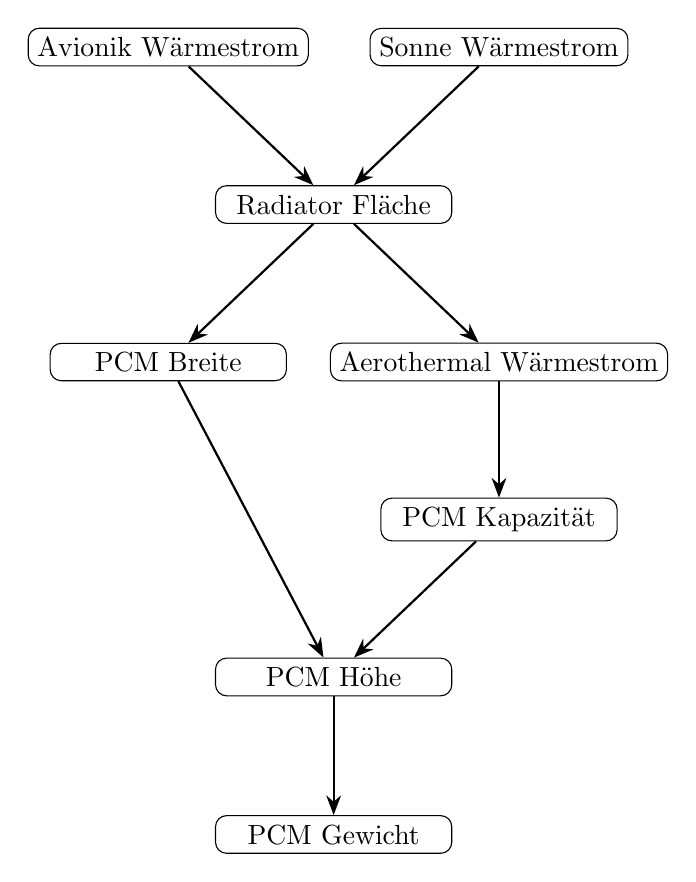
\begin{tikzpicture}[
    sibling distance=10em,
    every node/.style = {
      shape=rectangle,
      rounded corners,
      draw,
      align=center,
      minimum width=3cm
    },
    edge from parent/.style = {
      draw,
      ->,
      -{Stealth[length=0.25cm]},
      thick
    },
    arrow/.style = {
      ->,
      -{Stealth[length=0.25cm]},
      thick
    }
  ]

    % Top nodes
    \node (avionik) at (-2.1, 4) {Avionik Wärmestrom};
    \node (sonne)   at ( 2.1, 4) {Sonne Wärmestrom};

    % Radiator Fläche centered below
    \node (radiator) at (0, 2) {Radiator Fläche};

    % Children of Radiator
    \node (breite) at (-2.1, 0) {PCM Breite};
    \node (aerothermal) at (2.1, 0) {Aerothermal Wärmestrom};

    % PCM Kapazität as a separate node (not a child directly)
    \node (kapazitaet) at (2.1, -2) {PCM Kapazität};

    % PCM Höhe node below the center of breite and kapazitaet
    \node (hoehe) at (0, -4) {PCM Höhe};
    \node (gewicht) at (0, -6) {PCM Gewicht};

    % Arrows
    \draw[arrow] (avionik) -- (radiator);
    \draw[arrow] (sonne) -- (radiator);
    \draw[arrow] (radiator) -- (breite);
    \draw[arrow] (radiator) -- (aerothermal);
    \draw[arrow] (aerothermal) -- (kapazitaet);
    \draw[arrow] (breite) -- (hoehe);
    \draw[arrow] (kapazitaet) -- (hoehe);
    \draw[arrow] (hoehe) -- (gewicht);

  \end{tikzpicture}
  \caption{Dimensionierungs-Ablauf in der Vorauslegung}\label{fig:dimensionierung_ablauf}
\end{figure}

\begin{figure}[H]
  \centering
  \includegraphics[width=\linewidth]{../../Code/re_pr_during_flight.pdf}\label{fig:re_pr_flugsimulation}
  \caption{Reynolds- und Prandtlzahl während kritischer Phase im Flug}
  \includegraphics[width=\linewidth]{../../Code/pcm_radiator_hybrid_heatflux_nosim.pdf}\label{fig:pcm_waermestrom_vorauslegung}
  \caption{PCM Wärmestrom während Flug}
\end{figure}

\newpage

\section{Thermales Interface}\label{thermalesInterface}

Hier gehts jetzt um wie die wärme verteilt und abtransportiert wird. Laut~\cite{Xingcun-2011} seite 35 geht die meiste Wärme in die PCB.

\newpage

\subsection{Thermal Straps}\label{thermalstraps}

Um das \ac{pcb} mit der Heatpipe zu verbinden werden Thermal Straps aus verschiedenen Materialien analysiert.
Thermal Straps sind flexible Verbindungsteile die Wärmebrücken zwischen mehreren Bauteilen gewehrleisten.
Wegen der hohe Wärmeleitzahl von \ac{pgs} und bedonders für Thermal Straps wichtigen Flexibilität, sind diese eine interessante Option.
Ein Nachteil von \ac{pgs} ist die geringe Dicke und der daraus resultierende geringe Querschnitt, welcher trotz hoher Wärmeleitzahl zu hoher Wärmestromdichte und stärkerer Temperaturerhöhung führen kann.
Im Vergleich mit herkömmlichen Materialien wie Aluminium und Kupfer soll ein Vergleich gezogen werden.

\begin{figure}[H]
  \centering
  \includegraphics[width=\textwidth]{thermal_straps_commercial.png}
  \caption{Kommerzeill erhältliche Thermal Straps aus Graphen, Kupfer und Aluminium~\cite{Thermal-Straps}}\label{fig:thermalstraps_commercial}
\end{figure}

\newpage

%recoverytemperatur wahrscheinlich richtig noch recherchieren

% ----------- Diskussion & Schlussfolgerungen----------------------------------------
\newpage
\chapter{Simulation}\label{chap:Simulation}

Um die Ergebnisse der Vorauslegung zu verifizieren wurde mithilfe ANSYS Fluent sowohl das Verhalten des \ac{pcm}, als auch die
aerodynamische Aufheizung simuliert.

\section{PCM}\label{sec:sim_pcm}

Für die Simulation des \ac{pcm} wurde die in \ref{fig:pcm_struktur} dargestellte Struktur stark vereinfacht,
um trotz mangelnder Rechenressourcen gelöst werden zu können. Zuerst wurde das \ac{pcm} in der Symmetrieebene
zu einem zweidimensionalen Problem vereinfacht. Im nächsten Schritt wurde nur die mittlere Zelle aus der Ebene unter der Annahme,
dass das System symmetrisch ist ausgewählt. Im letzten Schritt wurde die Zelle nochmal aufgrund von Symmetrie gespalten.

Anschließend wurde in ANSYS Mechanical das Mesh vollständig aus Tetraeder-Elementen erzeugt, wobei die Zellgröße so gewählt
wurde, dass die Aluminium-Wände 1-2 Zellen Tiefe haben. In dem Mesh \ref{fig:pcm_mesh} ist das \ac{pcm} in schwarz und das Aluminium
in rot dargestellt. Jeweils an der linken und rechten Kante, wurde aufgrund der anliegenden Zelle bzw. Spiegelung der Zelle eine
Symmetrie Randbedingung gewählt. Die untere Kante wurde als Wärmequelle angelegt und die obere Kante als adiabate Wand.

Die Wärmequelle ergibt sich aus der Seitenfläche der \ac{pcm} Struktur, bestimmt in \ref{sec:pcm}, und dem Avionik Wärmestrom zu
$\frac{\SI{40}{\watt}}{\left(\SI{6,749}{\centi\meter}\right)^2} = \SI{8782}{\watt\per\meter\squared}$.
Da ANSYS Fluent bei zweidimensionalen Simulationen eine Referenztiefe von \SI{1}{m} verwendet, konnte der spezifische Wärmestrom
der Quelle direkt verwendet werden.

Die Thermodynamischen Eigenschaften von n-Eicosan sind aufgeführt in Tabelle \ref{tab:eicosane_data}.
Das temperaturabhängige Verhalten der spezifischen Wärmekapazität kann den Graphen \ref{fig:pcm_effective_cp} und \ref{fig:pcm_sensible_cp}
entnommen werden.

\begin{figure}[!htb]
    \centering
    \begin{subfigure}[t]{0.7\textwidth}
        \centering
        \includegraphics[height=9cm]{ansyspost/pcm/40WPCM_struktur.png}
        \caption{\ac{pcm} Struktur}\label{fig:pcm_struktur}
    \end{subfigure}
    \hfill
    \begin{subfigure}[t]{0.15\textwidth}
        \centering
        \includegraphics[height=9cm]{ansyspost/pcm/2DPCM_mesh.png}
        \caption{\ac{pcm} Mesh}\label{fig:pcm_mesh}
    \end{subfigure}
    \caption{\ac{pcm} Struktur und vereinfachtes Mesh}\label{fig:pcm_geometrien}
\end{figure}

\begin{table}[H]

  \centering
  \caption{Stoffdaten für n-Eicosan}\label{tab:eicosane_data}

  \begin{tabular}{lll}

    \toprule[1pt]
    Solidus Temperatur & $T_{\text{solidus}}$ & \SI{309}{\kelvin}~\cite{NIST} \\

    \midrule[0.5pt]
    Liquidus Temperatur & $T_{\text{liquidus}}$ & \SI{311}{\kelvin}~\cite{NIST} \\

    \midrule[0.5pt]
    Spezifische Wärmekapazität bei\\konstantem Druck der\\Flüssigphase & $c_{p,\text{liquid}}$ & \SI{2350.05}{\joule\per\kilogram\per\kelvin}~\cite{NIST} \\

    \midrule[0.5pt]
    Spezifische Wärmekapazität bei\\konstantem Druck der\\Feststoffphase & $c_{p,\text{solid}}$ & \SI{2132.4}{\joule\per\kilogram\per\kelvin}~\cite{NIST} \\

    \midrule[0.5pt]
    Dichte der Flüssigphase & $\rho_{\text{solid}}$ & \SI{910}{\kilogram\per\cubic\meter}~\cite{Nazarychev-2022} \\

    \midrule[0.5pt]
    Dichte der Feststoffphase & $\rho_{\text{liquid}}$ & \SI{769}{\kilogram\per\cubic\meter}~\cite{Nazarychev-2022} \\

    \midrule[0.5pt]
    Wärmeleitfähigkeit der Flüssigphase & $\lambda_{\text{liquid}}$ & \SI{0.1505}{\watt\per\meter\per\kelvin}~\cite{Benbrika-2020} \\

    \midrule[0.5pt]
    Wärmeleitfähigkeit der Feststoffphase & $\lambda_{\text{solid}}$ & \SI{0.4248}{\watt\per\meter\per\kelvin}~\cite{Stryker-1990} \\

    \midrule[0.5pt]
    Wärmeausdehnungskoeffizient & $\beta$ & \SI{0.0009}{\per\kelvin}~\cite{Benbrika-2020} \\

    \midrule[0.5pt]
    Spezifische Schmelzenthalpie & $h_{\text{fus}}$ & \SI{240998.86}{\joule\per\kilogram}~\cite{NIST} \\

    \bottomrule[1pt]
  \end{tabular}
\end{table}

\begin{figure}[H]
  \centering
  \includegraphics[width=\linewidth]{../../Code/eicosane_cpvst_total.pdf}
  \caption{Effektive spezifische Wärmekapazität von n-Eicosan}\label{fig:pcm_effective_cp}
\end{figure}

\begin{figure}[H]
  \centering
  \includegraphics[width=\linewidth]{../../Code/eicosane_cpvst_sensible.pdf}
  \caption{Sensible spezifische Wärmekapazität von n-Eicosan}\label{fig:pcm_sensible_cp}
\end{figure}

Die Simulation wurde mit dem Pressure-Based Solver~\cite{akamcae-udf} als transiente Simulation über 120000 Zeitschritte mit einer Zeitschrittgröße von \SI{0,01}{\second} durchgeführt
um die vollständige Flugdauer mit \SI{1200}{\second} zu simulieren.
Des weiteren wurde das Energiemodell eingeschaltet~\cite{akamcae-udf}, das Viskositätsmodell als Laminar angenommen~\cite{akamcae-udf} und das Phasenwechselmodell aktiviert~\cite{akamcae-udf}.
Neben den bereits erläuterten \ac{pcm} Eigenschaften wurde für das Aluminium eine Dichte von $\rho = \SI{2719}{\kilogram\per\meter\cubed}$,
eine spezifische Wärmekapazität von $c_p = \SI{871}{\joule\per\kilogram\kelvin}$ und eine Wärmeleitfähigkeit von $\lambda = \SI{202.4}{\watt\per\meter\kelvin}$
eingestellt.

Abbildung \ref{fig:approximierte_beschleunigung} zeigt das Beschleunigungsprofil, welches in der Simulation verwendet wurde. Zu beachten
ist, dass Beschleunigungsspitzen durch den Fallschirm, wie sie in~\ref{fig:acceleration_over_time} gesehen
werden können, ignoriert werden, da diese durch mangelhafte Genauigkeit der Fallschirm Modellierung resultieren.

\begin{figure}
  \centering
  \includegraphics[width=\linewidth]{../../Code/approximate_acceleration_over_time.pdf}
  \caption{Approximiertes Beschleunigungsprofil}\label{fig:approximierte_beschleunigung}
\end{figure}

Da die ANSYS Fluent Transient Table Funktion (Native Funktion für transiente Randbedingungen mit Profilen) keine transiente Gravitation
unterstützt, wurde diese und die globale Beschleunigung deaktiviert.
Stattdessen wurde die Beschleunigung über den Quellterm der Boussinesq-Approximation in der \ac{udf} implementiert. Die Funktion ist in
\ref{lst:udf_bossinesque} zu sehen.

Als Scheme wurde SIMPLE verwendet~\cite{akamcae-udf}, für die Gradienten Least Squares Cell Based~\cite{akamcae-udf}, für Druck Second Order~\cite{akamcae-udf} und für Impuls und Energie
Second Order Upwind~\cite{akamcae-udf}. Die Unterrelaxationsfaktoren wurden durch experimentelle Ermittlung anhand der Residuen zu 0,3 für Druck, 1 für Dichte
und Körperkräfte, 0,5 für Impuls und 0,9 für sowohl Flüssigkeitsanteil als auch Energie gewählt.

\begin{figure}
    \centering

    % Left figure
    \begin{minipage}[t]{0.485\textwidth}
        \centering
        \setlength{\tabcolsep}{1pt} % reduce subfigure spacing
        % Legend vertically centered & with extra space to right
        \begin{subfigure}[t]{0.16\textwidth}
            \centering
            \raisebox{0.7\height}{\includegraphics[height=0.2\textheight]{ansyspost/pcm/liquid-fraction-legend.png}}
        \end{subfigure}%
        \hspace{2mm}% extra space between legend and first image
        \begin{subfigure}[t]{0.2\textwidth}
            \centering
            \includegraphics[height=0.5\textheight]{ansyspost/pcm/liquid-fraction-300.png}
            \caption{\SI{300}{\second}}\label{fig:liquid_fraction_300}
        \end{subfigure}%
        \begin{subfigure}[t]{0.2\textwidth}
            \centering
            \includegraphics[height=0.5\textheight]{ansyspost/pcm/liquid-fraction-600.png}
            \caption{\SI{600}{\second}}\label{fig:liquid_fraction_600}
        \end{subfigure}%
        \begin{subfigure}[t]{0.2\textwidth}
            \centering
            \includegraphics[height=0.5\textheight]{ansyspost/pcm/liquid-fraction-900.png}
            \caption{\SI{900}{\second}}\label{fig:liquid_fraction_900}
        \end{subfigure}%
        \begin{subfigure}[t]{0.2\textwidth}
            \centering
            \includegraphics[height=0.5\textheight]{ansyspost/pcm/liquid-fraction-1200.png}
            \caption{\SI{1200}{\second}}\label{fig:liquid_fraction_1200}
        \end{subfigure}
        \caption{Flüssigkeitsanteil Konturen. Die Legende bezieht sich auf~\ref{fig:liquid_fraction_1200}}
        \label{fig:liquid_frac_kontur}
    \end{minipage}
    \hspace{2mm} % small horizontal space
    % Right figure
    \begin{minipage}[t]{0.485\textwidth}
        \centering
        \begin{subfigure}[t]{0.16\textwidth}
            \centering
            \raisebox{0.7\height}{\includegraphics[height=0.2\textheight]{ansyspost/pcm/temperature-legend.png}}
        \end{subfigure}%
        \hspace{2mm}% extra space between legend and first image
        \begin{subfigure}[t]{0.2\textwidth}
            \centering
            \includegraphics[height=0.5\textheight]{ansyspost/pcm/static-temperature-300.png}
            \caption{\SI{300}{\second}}\label{fig:temperatur_300}
        \end{subfigure}%
        \begin{subfigure}[t]{0.2\textwidth}
            \centering
            \includegraphics[height=0.5\textheight]{ansyspost/pcm/static-temperature-600.png}
            \caption{\SI{600}{\second}}\label{fig:temperatur_600}
        \end{subfigure}%
        \begin{subfigure}[t]{0.2\textwidth}
            \centering
            \includegraphics[height=0.5\textheight]{ansyspost/pcm/static-temperature-900.png}
            \caption{\SI{900}{\second}}\label{fig:temperatur_900}
        \end{subfigure}%
        \begin{subfigure}[t]{0.2\textwidth}
            \centering
            \includegraphics[height=0.5\textheight]{ansyspost/pcm/static-temperature-1200.png}
            \caption{\SI{1200}{\second}}\label{fig:temperatur_1200}
        \end{subfigure}
        \caption{Konturen der statischen Temperatur. Die Legende bezieht sich auf~\ref{fig:temperatur_1200}}
        \label{fig:static_temperature_kontur}
    \end{minipage}

\end{figure}

In Abbildung \ref{fig:static_temperature_kontur} und \ref{fig:liquid_frac_kontur} kann man jeweils die Lösung des Flüssigkeitsanteils
und der statischen Temperatur zu mehreren Zeitschritten sehen. Man kann dort deutlich erkennen, wie das \ac{pcm} von der Wärmequelle aus
schmilzt. Besonders an der Aluminiumlamelle bildet sich eine beschleunigte Konvektion die jedoch nach unten fließt und durch das aufsteigende
\ac{pcm} in der Mitte der Zelle angetrieben wird. Im Vektorfeld \ref{fig:pcm_vectoren_stitched} kann man den dadurch entstandenen Wirbel sehen.

Besonders interessant ist, dass wie in \ref{fig:static_temperature_kontur} zu erkennen ist, die Temperatur an der Quelle auf bis zu \SI{336}{\kelvin}
steigt. Demnach würde mittels der Thermalen Schnittstelle aus \ref{sec:thermale_schnittstelle} die Gehäusetemperatur der Avionik-Bauteile mit
$T_C = \SI{384,17}{\kelvin}$ über die zuverlässige Temperatur steigen.

\begin{lstlisting}[language=C, float, caption={Boussinesq-Approximation des Auftriebs im \ac{pcm} in der \ac{udf} eicosane.c}, label={lst:udf_bossinesque}]
//Y-momentum source
DEFINE_SOURCE(Boussinesq_momentum_source,cell,thread,dS,eqn)
{
	double Temp, source, acc;
	Temp=C_T(cell,thread);

	double t = CURRENT_TIME;

	if (t < 20)
		acc = 34.81;
	else if (t < 50)
		acc = 109.81;
	else if (t < 150)
		acc = 19.62;
	else
		acc = 9.81;

	source=-Rol_pcm*acc*TEC*(Temp-Tr);  //negative for -Y down
	dS[eqn]=-Rol_pcm*acc*TEC; 			//negative for -Y down
	return source;
}
\end{lstlisting}

\begin{figure}
  \centering
  \includegraphics[height=0.4\textheight]{ansyspost/pcm/velocity-vector-close-stitched-900.png}
  \caption{Geschwindigkeitsvektoren der Konvektionswirbel einer, durch Nachbearbeitung, vervollständigten Zelle
  bei \SI{900}{\second}. Darstellung der weiteren Zeitschritte ist in~\ref{fig:pcm_static_temperature_kontur} zu finden.}\label{fig:pcm_vectoren_stitched}
\end{figure}

\section{Aerodynamische Aufheizung}\label{sec:sim_aerodynamisch}
Die Simulation der aerodynamischen Aufheizung wurde als stationäre Simulation mit dem Density-Based solver durchgeführt. Hierbei wurde
aufgrund der Rotationssymmetrie der Rakete im relevanten Bereich oberhalb der Finnen wieder eine zweidimensionale Simulation durchgeführt.
Als Viskositätsmodell wurde SST k-$\omega$~\cite{Irving-2021} gewählt und das Energiemodell aktiviert.
Die Luft wurde als Ideales Gas mit einer spezifischen Wärmekapazität von \SI{1006.43}{\joule\per\kilogram\kelvin},
einer Wärmeleitfähigkeit von \SI{0.0242}{\watt\per\meter\kelvin}, einer dynamischen Viskosität von \SI{1.7894e-5}{\kilogram\per\meter\second}
und einer molekularen Masse von \SI{28,966}{\kilogram\per\kilo\mole} modelliert.

Die Außenstruktur der Rakete besteht aus dem zylindrischen Hüllensegment und einem von-Kármán-Nasenprofil das analytisch
beschrieben wird:

\begin{equation*}
  \label{eq:karman_nase}
  x(t) = \frac{R}{\sqrt{\pi}} \cdot \sqrt{
  \cos^{-1}\left(1 - \frac{2t}{L} \right)
  - \frac{1}{2} \cdot \sin\left(2 \cdot \cos^{-1}\left(1 - \frac{2t}{L} \right) \right)
  }
  \quad \text{für } t \in [0, L]
\end{equation*}

Hierbei ist $x(t)$ der Radiusverlauf des rotationssymmetrischen Nasenprofils entlang der Längskoordinate $t$, beginnend an der Spitze $(t=0)$ bis zur Basis $(t=L)$.
Der maximale Radius an der Basis beträgt $R = \SI{125}{\milli\meter}$ und die Gesamtlänge der Nase $L = \SI{1250}{\milli\meter}$.
Dies entspricht dem Gesamtdurchmesser der Rakete von $D = \SI{250}{\milli\meter}$.

Das Mesh der Domäne wurde in ANSYS Mechanical vollständig aus Tetraeder-Elementen erstellt und ist samt Randbedingungen in \ref{fig:aussenstroemung_mesh} dargestellt.
Um die Grenzschicht-Anforderung aus \ref{eq:yplus} mit $y^+ \leq 1$ zu erfüllen, wurden Inflationsschichten an der Raketenwand eingefügt, die in \ref{fig:aussenstroemung_mesh_inflationlayers}
zu sehen sind. Die Höhe der ersten Schicht wurde experimentell erhalten \cite{Anderson-2017}

Die Vorauslegungwurde mit folgenden Werten durchgeführt:\\
- Isotherm auf: \SI{38}{\celsius}\\
- Avionik Abwärme: \SI{40}{W}\\
- \SI{1}{m} Kontourlänge\\
- Radiator Emissionsgrad: \SI{0,91}{} (AZ-93)\\
- Radiator Absorptionsgrad: \SI{0,15}{} (AZ-93)\\
- Icosane PCM\\
- Trajektoriensimulation\\
- \SI{1}{\kilo\watt\per\meter\squared} mit 50\% dutycycle durch Rotation der Rakete\\
Zu beachten ist, dass die Radiatorleistung konstant bleibt, da das System als isotherm mit einer
infinitesimalen Temperaturerhöhung über den Schmelzpunkt hinweg angenommen wird.\\
Als nächstes sieht man die Flugdaten

Speziell für die Strömungssimulationen welche keine Koppelung mit Festkörpern haben, wurde der Density-Based Solver ausgewählt und die
Simulation als 2D Steady State durchgeführt. Das Energiemodell wurde aktiviert und für das Viskositätsmodell~\cite{Irving-2021}

Die Umströmungssimulationen der Rakete wurden an \ac{maxq} orientiert, da es als Richtwert für Aerodynamische Aufheizung genommen werden kann.
Desweiteren ist der Wert unanhängig von der Vorauslegung, wodurch Ungenauigkeiten von dort getroffenen Annahmen vermieden werden.\\


als nächstes habe ich geschaut wo der maximale dynamische Druck erreicht wurde in der Vorauslegung. Die korrespondierenden Werte des Flugzustandes
habe ich dann als Boundery Conditions in der \ac{cfd}~Simulation genommen.
Um zu verifizieren, dass dort auch die maximale Aufheizung stattfindet, habe ich 1 Sekunden vorher und nachder
im Flug die BC's auch verwendet und einen Vergleich gezogen.\\
Maximaler dynamischer Druck: 112901.25708461029 Pa at 28.691 s\\
Entsprechender Flugzustand: 10244.138 m, 750.704 m/s, -51.587°C, 254.783 hPa mit entsprechender Luft Dichte \SI{0.4006}{kg/m^3}\\
Flugzustand bei 18.691 s \ac{maxq} - $\SI{10}{\second}$: 4274.387 m, 461.355 m/s, -12.784, 594.935 hPa mit entsprechender Luft Dichte \SI{0.7960}{kg/m^3}\\
Flugzustand bei 38.691 s \ac{maxq} + $\SI{10}{\second}$: 19758.652 m, 1189.968 m/s, -56.5°C, 56.93 hPa mit entsprechender Luft Dichte \SI{0.0915}{kg/m^3}\\
Flugzustand bei 48.7 s \ac{maxq} + $\SI{20}{\second}$: 32439.616 m, 1393.377 m/s, -43.269°C, 8.136 hPa mit entsprechender Luft Dichte \SI{0.01233001}{kg/m^3}\\
Da wie in~\ref{fig:spezifischer_waermestrom_maxQ_simulationen} zu sehen ist, der Zeitpunkt des maximalen dynamischen Druckes nicht im größten spezifischen
Wärmestrom resultiert, wurde mit der Simulation die den höheren spezifischen Wärmestrom ergeben hat, eine Lösungsfortsetzung durchgeführt um das Maximum zu finden.\\

\begin{figure}[H]
  \centering
  \includegraphics[width=\linewidth]{ansyspost/airflow/mesh_all.png}
  \caption{Darstellung der Außensströmungssimulation mit Meshstruktur in grau, velocity inlet in blau, pressure outlet in rot, Symmetrien in gelb und Partitionen der parallelisierung in lila}\label{fig:aussenstroemung_mesh}
\end{figure}

\begin{figure}[H]
  \centering
  \includegraphics[width=\linewidth]{ansyspost/airflow/mesh_inflation.png}
  \caption{Schichtaufdickungen des Mesh an der Rakete}\label{fig:aussenstroemung_mesh_inflationlayers}
\end{figure}

\begin{figure}[H]
  \centering
  \includegraphics[width=\linewidth]{../../Code/maxQ_compare_heatflux.pdf}
  \caption{Spezifischer Wärmestrom an der Außenhaut bei maximalem dynamischen Druck, sowie \SI{10}{s} davor, danach und \SI{20}{s} danach}\label{fig:spezifischer_waermestrom_maxQ_simulationen}
\end{figure}

\begin{figure}[H]
  \centering
  \includegraphics[width=\linewidth]{../../Code/maxQ_compare_yplus.pdf}
  \caption{y+ Wert an der Außenhaut bei \ac{maxq}, sowie \SI{10}{s} davor, danach und \SI{20}{s} danach}\label{fig:yplus_maxQ_simulationen}
\end{figure}

\begin{figure}[H]
  \centering
  \includegraphics[width=\linewidth]{../../Code/pcm_radiator_hybrid_heatflux_with_sim.pdf}
  \caption{PCM Wärmestrom während Flug mit Simulationsergebnissen und Fit Kurve}\label{fig:pcm_waermestrom_sim}
\end{figure}

Fitted Gaussian parameters:
a=12454028.32, b=32.87, c=550.50, d=-12446646.16

\begin{figure}[H]
    \centering

    \begin{subfigure}{\textwidth}
        \centering
        \includegraphics[height=0.23\textheight]{ansyspost/airflow/maxQ-temperature-contour.png}
        \caption{Statische Temperaturkontur der Luft}
        \label{fig:maxQ_temp_contour}
    \end{subfigure}

    \begin{subfigure}{\textwidth}
        \centering
        \includegraphics[height=0.23\textheight]{ansyspost/airflow/maxQ-mach-contour.png}
        \caption{Machzahlkontur der Luft}
        \label{fig:maxQ_mach_contour}
    \end{subfigure}

    \caption{\texorpdfstring{\ac{maxq}}{max Q} Konturen der Luft}
    \label{fig:maxQ_konturen}
\end{figure}

% ----------- Diskussion & Schlussfolgerungen----------------------------------------
\newpage
\chapter{Discussion and conclusions}
\label{chap:conclusion}

\section{Discussion about including pictures}


% ----------- Ausblick --------------------------------------------------------------
\newpage
\chapter{Zusammenfassung und Ausblick}
\label{chap:Ausblick}
\pagestyle{OnlySection}		% wie ganz oben definiert

Beispielliteraturverweise: 

\begin{enumerate}
	\item Fachzeitschrift
	\item Internetquelle
	\item Buch 
	\item Vorlesungsskript
\end{enumerate}

Anmerkung: Es gibt verschiedene Referenzierungsstile 


% ----------- Literatur -------------------------------------------------------------
\newpage
\renewcommand{\bibname}{Literaturverzeichnis}

\bibliography{Bibliography/quellen.bib}
\bibliographystyle{plain}%{unsrt}{abbrv}{abbrvnat}{unsrt}

\newpage

%----------- Anhang -----------------------------------------------------------------
\chapter*{Appendix}
\label{chapter:Appendix}
\pagestyle{Appendix}
\addcontentsline{toc}{chapter}{Appendix}

\section*{Appendix A: Simulationsergebnisse}\label{Anh:simulation}

\begin{figure}[H]
    \centering

    \begin{subfigure}{\textwidth}
        \centering
        \includegraphics[height=0.23\textheight]{ansyspost/airflow/maxQminus10-temperature-contour.png}
        \caption{maxQ -\SI{10}{\second}}
        \label{fig:maxQminus10_temp_contour}
    \end{subfigure}

    \begin{subfigure}{\textwidth}
        \centering
        \includegraphics[height=0.23\textheight]{ansyspost/airflow/maxQplus10-temperature-contour.png}
        \caption{maxQ +\SI{10}{\second}}
        \label{fig:maxQplus10_temp_contour}
    \end{subfigure}

    \begin{subfigure}{\textwidth}
        \centering
        \includegraphics[height=0.23\textheight]{ansyspost/airflow/maxQplus20-temperature-contour.png}
        \caption{maxQ +\SI{20}{\second}}
        \label{fig:maxQplus20_temp_contour}
    \end{subfigure}

    \caption{Statische Temperaturkontur der Luft}
    \label{fig:airflow_temp_contour_continued}
\end{figure}

\begin{figure}[H]
    \centering

    \begin{subfigure}{\textwidth}
        \centering
        \includegraphics[height=0.23\textheight]{ansyspost/airflow/maxQminus10-mach-contour.png}
        \caption{maxQ -\SI{10}{\second}}
        \label{fig:maxQminus10_mach_contour}
    \end{subfigure}

    \begin{subfigure}{\textwidth}
        \centering
        \includegraphics[height=0.23\textheight]{ansyspost/airflow/maxQplus10-mach-contour.png}
        \caption{maxQ +\SI{10}{\second}}
        \label{fig:maxQplus10_mach_contour}
    \end{subfigure}

    \begin{subfigure}{\textwidth}
        \centering
        \includegraphics[height=0.23\textheight]{ansyspost/airflow/maxQplus20-mach-contour.png}
        \caption{maxQ +\SI{20}{\second}}
        \label{fig:maxQplus20_mach_contour}
    \end{subfigure}

    \caption{Machzahlkontur der Luft}
    \label{fig:airflow_mach_contour_continued}
\end{figure}

\begin{figure}[H]
    \centering

    \begin{subfigure}[t]{0.14\textwidth}
        \centering
        \raisebox{1\height}{\includegraphics[height=0.2\textheight]{ansyspost/pcm/vector-legend.png}}
    \end{subfigure}%
    \hspace{2mm}% extra space between legend and first image
    \begin{subfigure}[t]{0.2\textwidth}
        \centering
        \includegraphics[height=0.7\textheight]{ansyspost/pcm/velocity-vector-300.png}
        \caption{\SI{300}{\second}}\label{fig:velocity_vector_300}
    \end{subfigure}%
    \begin{subfigure}[t]{0.2\textwidth}
        \centering
        \includegraphics[height=0.7\textheight]{ansyspost/pcm/velocity-vector-600.png}
        \caption{\SI{600}{\second}}\label{fig:velocity_vector_600}
    \end{subfigure}%
    \begin{subfigure}[t]{0.2\textwidth}
        \centering
        \includegraphics[height=0.7\textheight]{ansyspost/pcm/velocity-vector-900.png}
        \caption{\SI{900}{\second}}\label{fig:velocity_vector_900}
    \end{subfigure}%
    \begin{subfigure}[t]{0.2\textwidth}
        \centering
        \includegraphics[height=0.7\textheight]{ansyspost/pcm/velocity-vector-1200.png}
        \caption{\SI{1200}{\second}}\label{fig:velocity_vector_1200}
    \end{subfigure}
    \caption{Konturen der statischen Temperatur. Die Legende bezieht sich auf~\ref{fig:temperatur_1200}}\label{fig:pcm_static_temperature_kontur}
\end{figure}

\section*{Appendix B: bla}
\label{Anh:bla2}

%------------------------------------------------------------------------------------
\end{document}